\chapter{DEMO CODES}

\section{Lists}
\begin{itemize}
	\item Create a specific data logging device for the given Electro Field Meter (EFM).
	\item Provide the required power supply to the field mill on-board the UAV. 
	\item Integrate the EFM to the payloads bay.

\end{itemize}

 \begin{description}
	\item[Ground stations] The most common procedure is to attract the lightnings to a tall tower fully monitored. When a thunderstorm is unchained near the tower, there are strong chances of lightnings hits, which can be studied. The main drawback is that the tower must be placed on a usually thunderstorms zone where attract lightnings don't represent a risk to humans lives. Used all-round the world.  
	\item[Rocket triggering] A rocket is launch with an electric wire attached to its bottom, when the atmosphere conditions are favourable for a lightning discharge. When te conductor hit the  charged cloud a lightning falls along the wire. Then is measured by the sensors on the ground. Rocket triggering method is currently used by the \textit{Lightning Research Group of Florida University} with great results.

\end{description}

\section{Short Tables}
%TAULES CURTES
\begin{table}[H]
	\centering
	\begin{tabular}{c p{14cm}}
		\toprule[2pt]
		\textbf{Feature} & \textbf{Description}                                                                                                                                                          \\ \midrule

		3                & \begin{tabular}[c]{@{}l@{}}\begin{minipage}[t]{\linewidth}
				UAV platform must be \textbf{fail-safe}. \\
				If it lose controlling signal coverage, must be able to \textbf{perform predefined manoeuvres} and \textbf{auto-land}. \\
				If a major controlling electronics failure happens, UAV, needs to have a \textbf{safe landing mechanism} such as a parachute.
		\end{minipage} \end{tabular}\vspace{0.3cm}                                                 \\
		4                & \begin{tabular}[c]{@{}l@{}}\begin{minipage}[t]{\linewidth}
				UAV platform must be able to carry \textbf{250g }of payload at least.
		\end{minipage}\end{tabular}\vspace{0.3cm}                                                                                                     \\
		5                & \begin{tabular}[c]{@{}l@{}}\begin{minipage}[t]{\linewidth}
				All payloads \textbf{sensor data} should be at least \textbf{stored} on board.
		\end{minipage}\end{tabular}\vspace{0.3cm}                                                                                                     \\
		\\ \bottomrule[2pt]
	\end{tabular}
	\caption{Project Requirements}
\end{table}



\section{Images}
\begin{figure}[H]
	\centering
	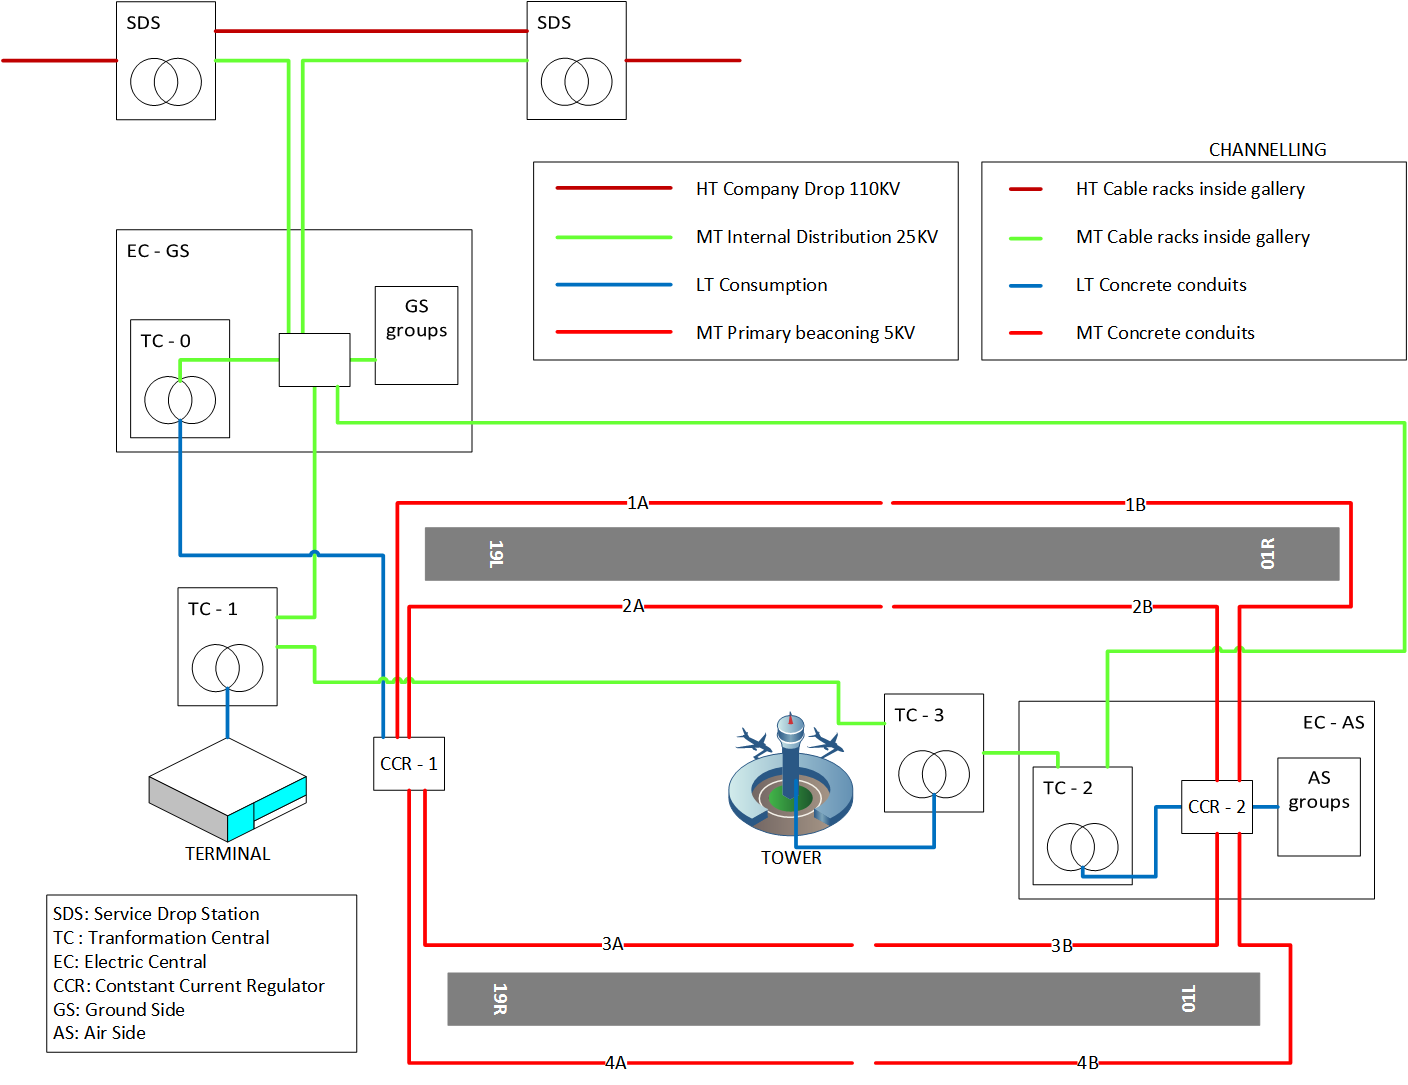
\includegraphics[clip, trim=0cm 0cm 0cm 0cm, width=0.5\textwidth]{./images/electric/esquema_electrico}
	\caption{General electric system scheme}
	\label{electricScheme}
\end{figure}

\section{PDF HORITZONTAL}
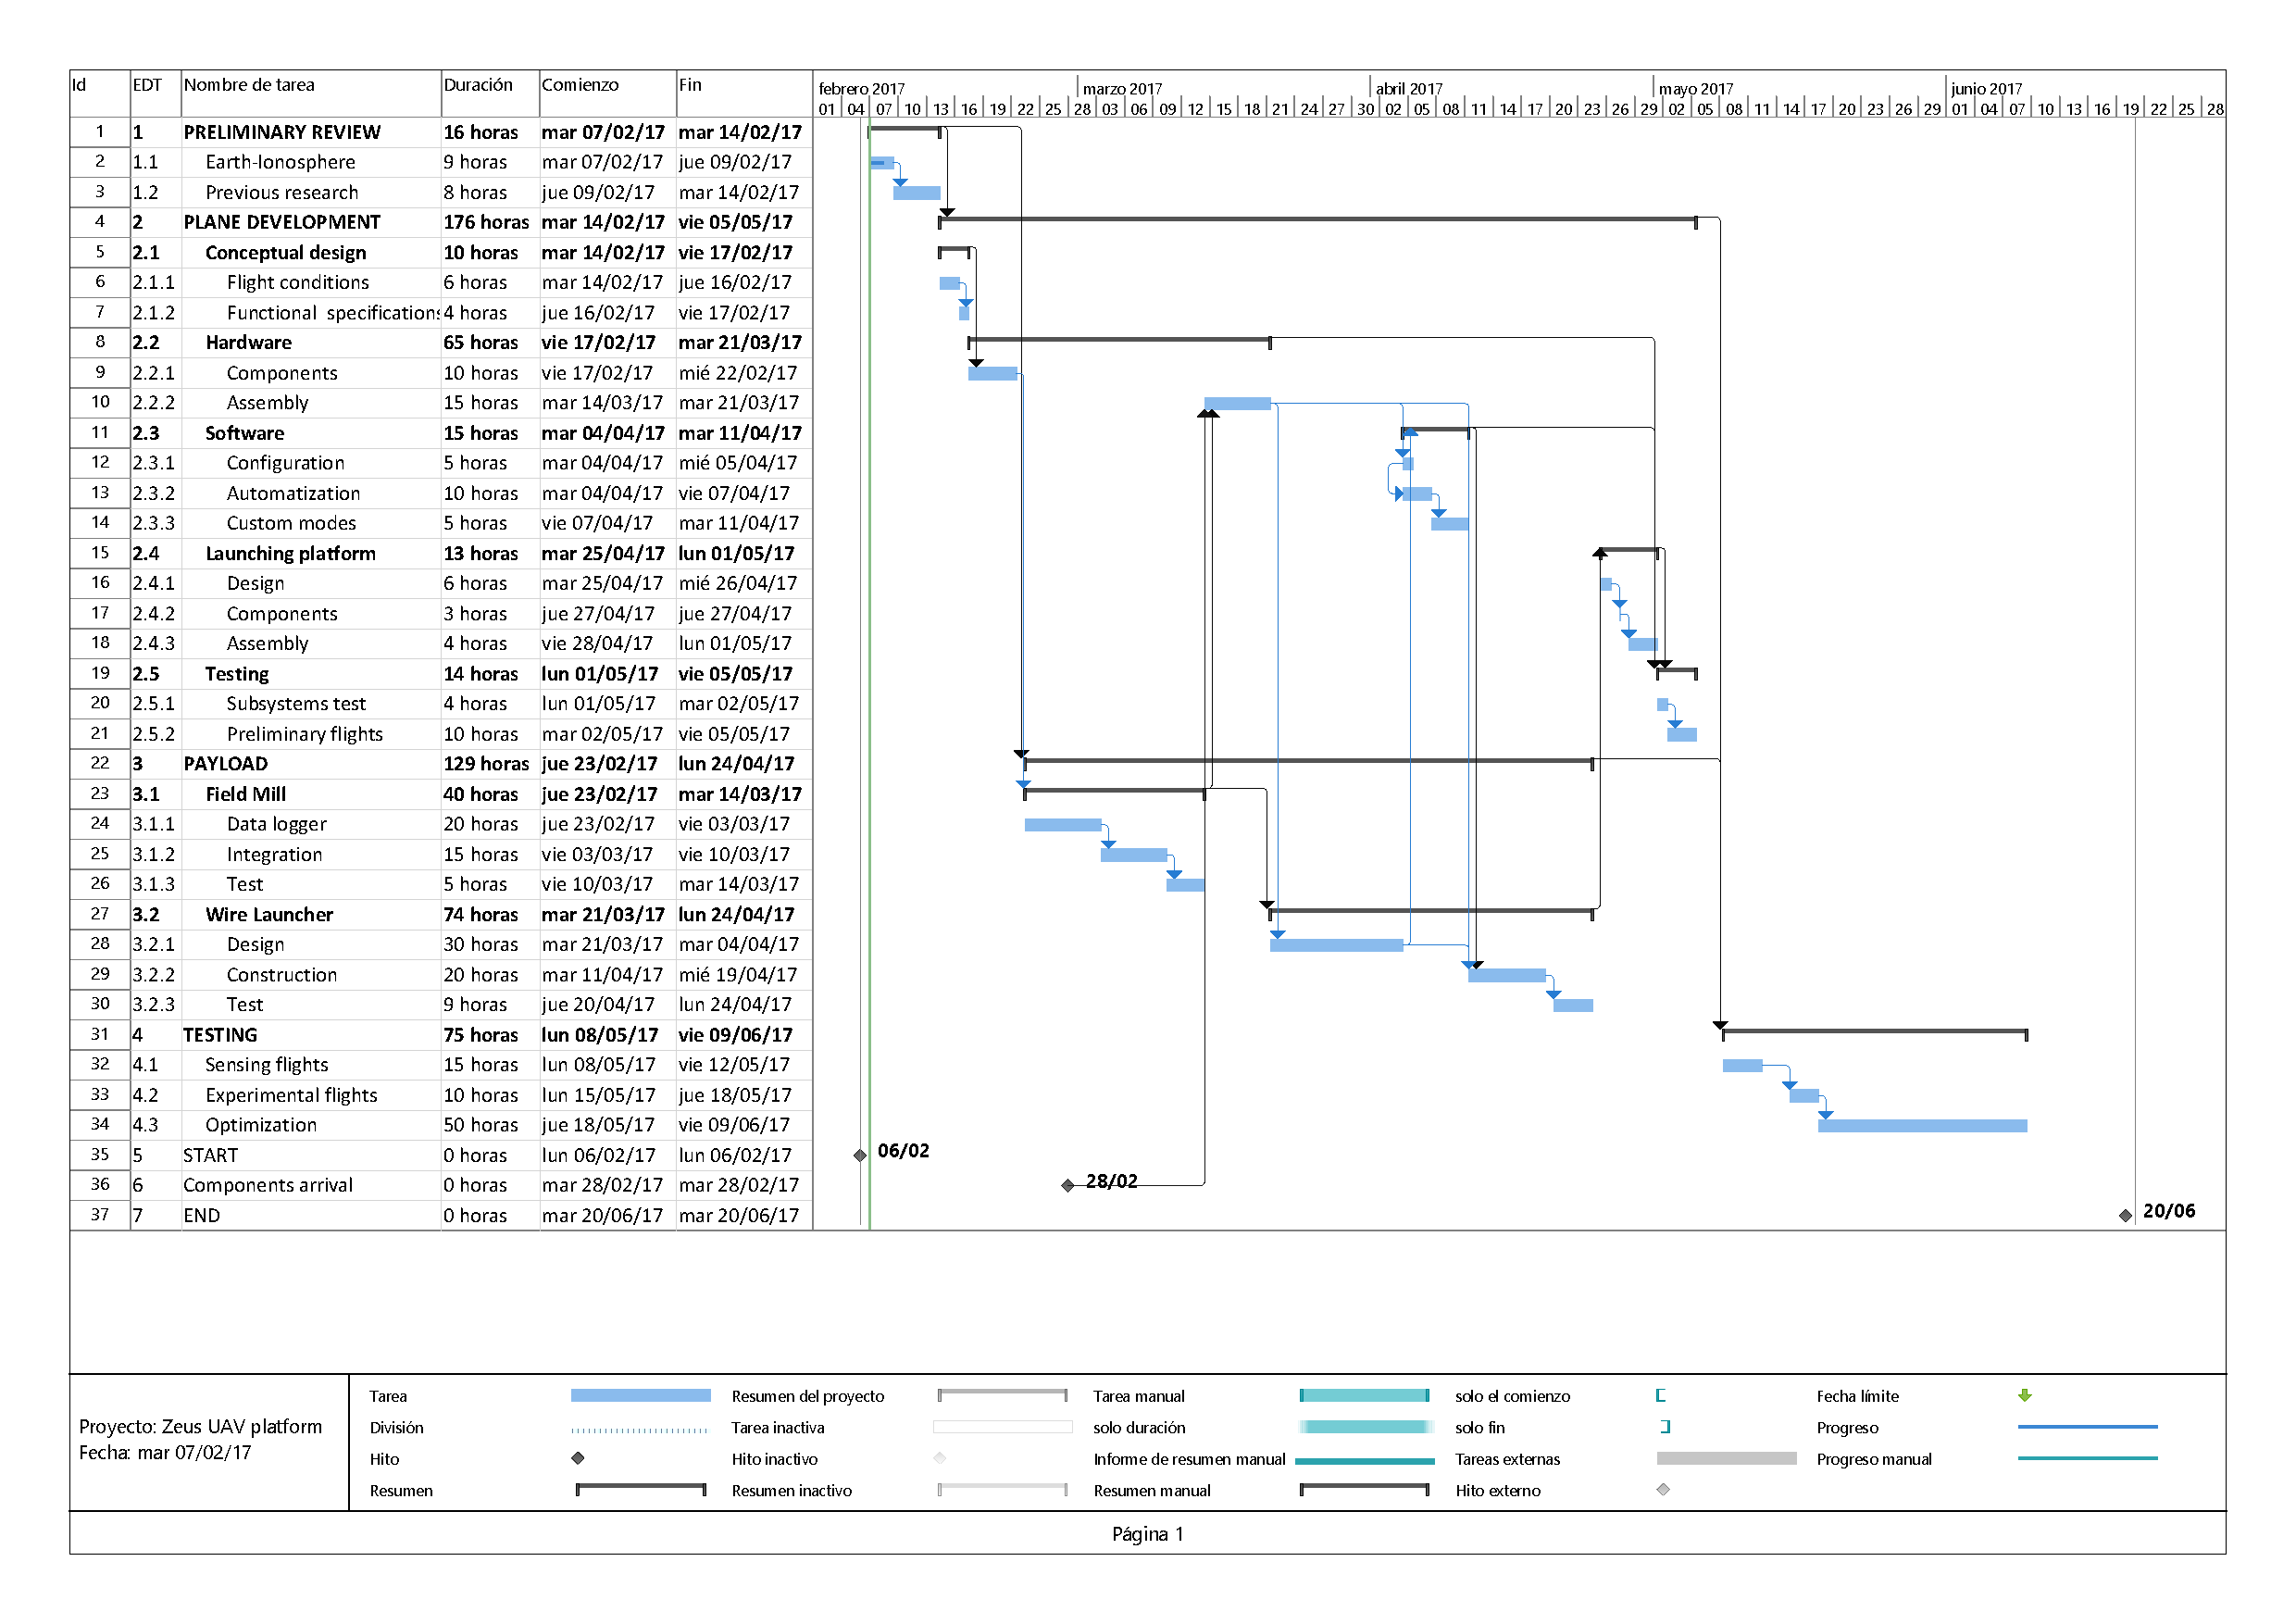
\includepdf[landscape=true]{./RAW/GANTT}
